\icode{E-MCH-SI-L2-260627-001}
如图所示，A、B两小球从相同高度同时水平抛出，经过时间t在空中相遇，若两球的抛出速度都变为原来的2倍，则两球从抛出到相遇经过的时间为\paren[]
      
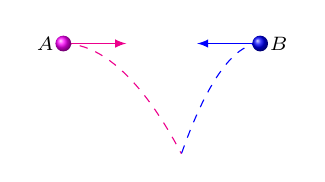
\begin{tikzpicture}[>=latex,font=\scriptsize]
    \draw[->,magenta] (0,2)node[left,black]{\(A\)}--++(.8,0);
    \draw[->,blue] (2.5,2)node[right,black]{\(B\)}--++(-.8,0);
    \draw[dashed,magenta] (0,2) parabola bend(0,2) (1.5,.6);
    \draw[dashed,blue] (2.5,2) parabola bend(2.5,2) (1.5,.6);
    \shade[ball color=magenta] (0,2) circle(.1);
    \shade[ball color=blue] (2.5,2) circle(.1);
\end{tikzpicture}
\begin{choices}
    \item \(t\)
    \item \(\frac{\sqrt{2}}{2}t\)
    \item \(\frac{t}{2}\)
    \item \(\frac{t}{4}\)
\end{choices}
\begin{answer}
    C
\end{answer}